\documentclass{beamer}
\mode<presentation>{\usetheme{classic}
\setbeamercovered{transparent}}
\usepackage[T1]{fontenc}
\usepackage{ifpdf}
\usepackage{graphicx}
\usepackage{color}

\newcommand{\tbf}{\textbf}
\newcommand{\ds}{\displaystyle}
\newcommand{\ra}{\rightarrow}

\ifpdf
\hypersetup{pdfpagemode=FullScreen}
\fi

\title{\tbf{Dirty money: \\ Feature Selection Using AdaBoost}}
\author{Silvia, Jasper \& Nimrod}
%\subject{bmeps}
\begin{document}

\frame{\titlepage}
\section[Outline]{}
\frame{\tableofcontents}


% \beamertemplateshadingbackground{yellow!50}{magenta!50}


\section{Introduction}
	\frame{
		\frametitle{What and why?}
		\hspace*{8pt}Recognize the dirty bills from the clean once\\
		\vspace{10pt}\pause
		\hspace*{8pt}Euro bills are manufactured all over europe,\\ 
		\hspace*{8pt}with different paper and ink, which makes sorting hard\\
		\vspace{10pt}
		\hspace*{8pt}for example, usa has 2 bill factories and one paper factory\\
	}

	\frame{ 
		\frametitle{some facts} 
		\begin{itemize}
		\item Bills return to the bank 2 or 3 times a year (1.1 billion bills a year) 
		\item 30\% of 5-euro bills is destroyed
		\item current detection of dirty bills works with reflection of light
		\item best sorting machines destoys 15\% of all bills in order to destroy 95%
		of the dirty bills
		\item value of good bills that are destoyed in holland is 1.5 million euro
		\end{itemize}
	}  	
	
\section{Previous work}
	\subsection{How does the DNB do it?}
		\frame{
  			\frametitle{DNB approach}
  			\hspace*{8pt} Reflection of light on small area near water mark area\\
  			\vspace{10pt}\pause
  			\hspace*{8pt} Results:
			\begin{itemize}
			\item  5\% dirty bills error 
			\item 30\% clean bills error
			\end{itemize}
  		}
	\subsection{By Molenaar, Nusselder \& Stefanov}
		\frame{
  			\frametitle{MNS approach}
  			\hspace*{8pt} Learn eigen money using PCA\\
  			\vspace{10pt}\pause
  			\hspace*{8pt} Results (what are the right numbers?):
			\begin{itemize}
			\item   5 euro: 10\%  7\%  
			\item  10 euro:  8\%  5\%  
            \end{itemize} 
  		}
	\subsection{By Jan-Mark Geusebroek}
		\frame{
  			\frametitle{JM approach}
  			\hspace*{8pt} Pre-processing: 
			\begin{itemize}
				\item bills alligned  
				\item non-linear reflection
				\item water-mark region extracted
            \end{itemize} 
  			\hspace*{8pt} Learn eigen-money on water mark region\\
  			\vspace{10pt}\pause
  			\hspace*{8pt} Results:
			\begin{itemize}
			\item   5 euro:  3\%  0\% 
			\item  10 euro: 16\%  6\%  
			\end{itemize}
  		}

  		
\section{Our approach}
	\subsection{Task redefined}
		\frame{
  			\frametitle{The task}
			\hspace*{8pt} Improve classification of 5 and 10 euro bills\\
			\vspace{10pt}\pause
			\hspace*{8pt} new data set:\\
			\hspace*{8pt} Euro 5 and 10\\
			\hspace*{18pt} $\approx400$ banknotes per class\\
			\hspace*{18pt} $\approx250$ fit, $\approx150$ unfit
		}
		\frame{
  			\frametitle{Classifiers}
			\hspace*{8pt} Three different stong classifiers built fron weak classifiers\\
			\vspace{10pt}\pause
			\begin{itemize}
				\item Haar 
				\item PCA  
				\item intensity \& edge  
			\end{itemize}
			\hspace*{8pt} combined into one final classifier
		}

	\subsection{Intensity \& edge} 
		\frame{
			\frametitle{Intensity \& edge}
			\hspace*{8pt}Intensity approach is inspired by current approach DNB\\
			\vspace{10pt}
			\hspace*{8pt}Can be (easily) computed by the average intansity of a bill\\
			\vspace{10pt} \pause
			\hspace*{8pt}Edge approach is inspired by idea that used bill have more folds
			nad wrinkles\\ 
			\vspace{10pt}
			\hspace*{8pt}Can be computed by the sum of edge-points from a canny edge
			filter 
		}
	\frame{
		\frametitle{Intensity \& edge}
			\begin{figure}[H]
				\begin{center}
					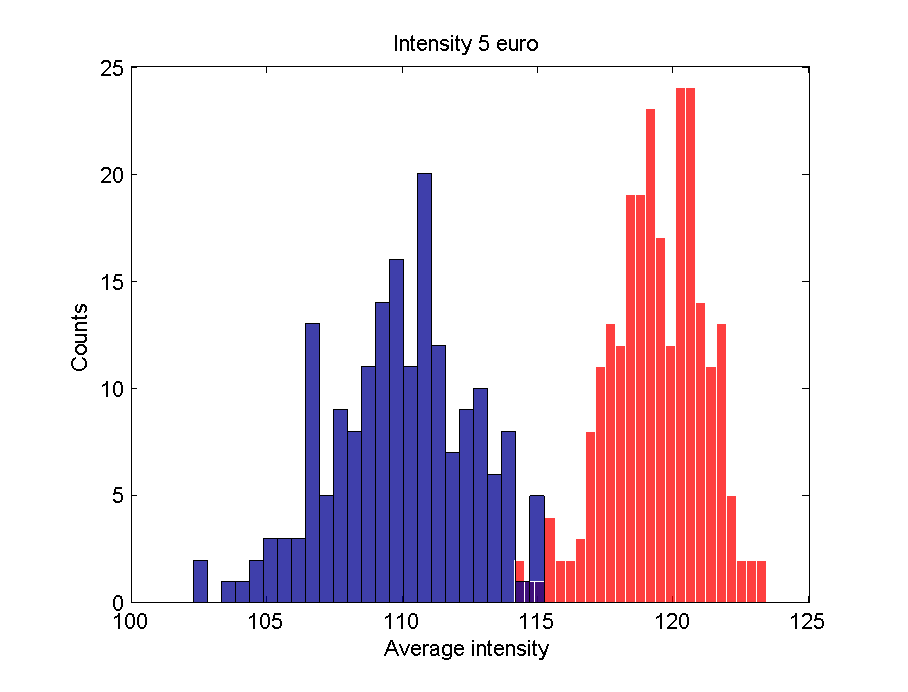
\includegraphics[width=5cm]{img/neur05int.eps}
					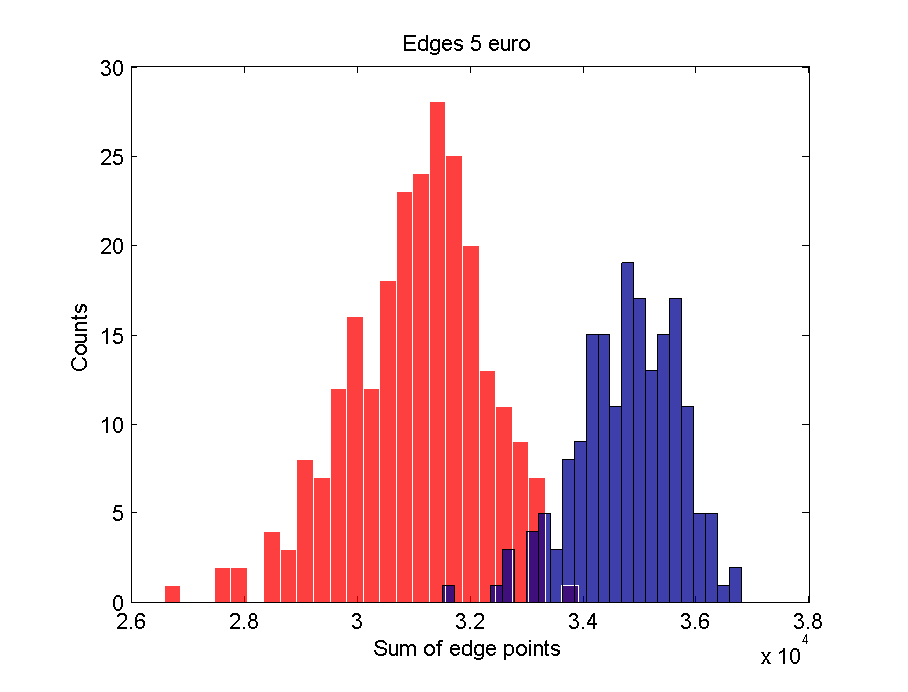
\includegraphics[width=5cm]{img/neur05edge.eps} \\
					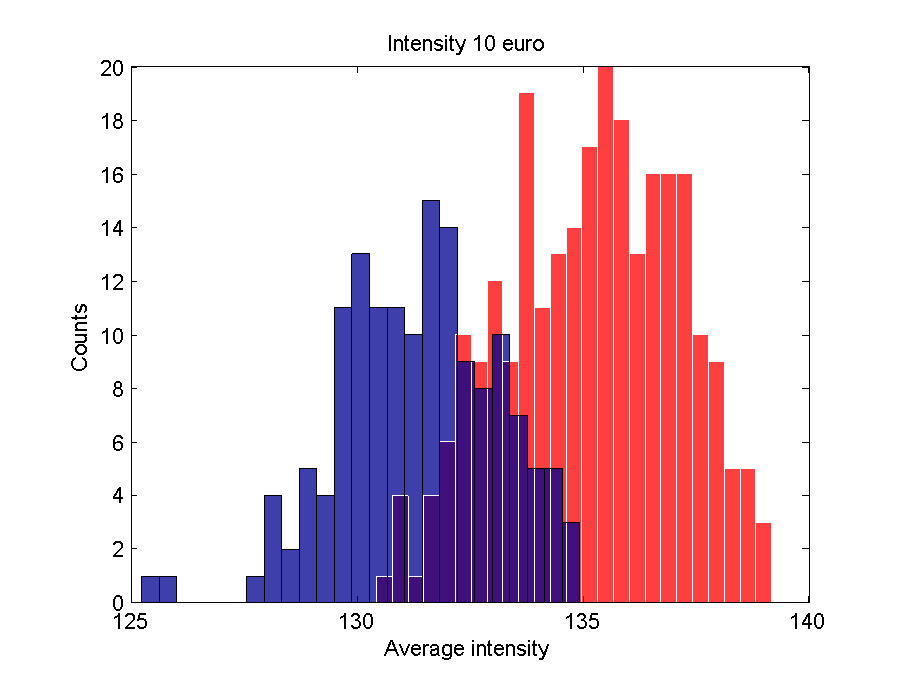
\includegraphics[width=5cm]{img/neur10int.eps}
					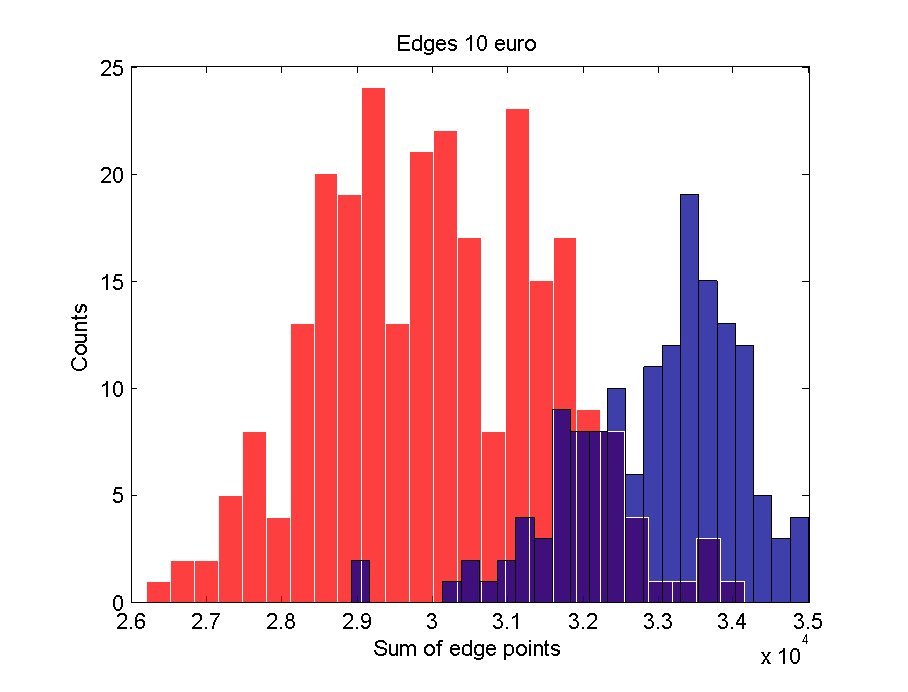
\includegraphics[width=5cm]{img/neur10edge.eps} \\
				\end{center}
			\end{figure}
	}

	\subsection{Adaboost} 
		\frame{
			\frametitle{Adaboost}
			\hspace*{8pt}Adaboost is used to combine weak classifiers into a strong classifier\\
		}

\section{Experiments \& results}
	\frame{
		\frametitle{Results Haar}
		\hspace*{8pt}Haar
	}
	\frame{
		\frametitle{Results PCA}
		\hspace*{8pt}PCA
	}
	\frame{
		\frametitle{Results intensity \& edge}
		\hspace*{8pt}Intensity \& edge
	}
	\frame{
		\frametitle{Results combined}
		\hspace*{8pt}Combined classifier
	}

\section{Conclusion}
	\frame{
		\frametitle{conclusion}
		\hspace*{8pt}conclusion
	}

\section{future work} 
	\frame{
		\frametitle{future work}
		\hspace*{8pt}future work
	}
\end{document}